\label{sec:2-task1}
There are various software packages or programmatic methods available to build and analyse networks. Throughout this project we work mainly with \PY and the \textsc{NetworkX} module. Furthermore, there are a lot of sources from which you can obtain and integrate PPI data, other than creating new experimental results. Current databases are distinguished in primary or predicting, depending on whether they just provide evidence or combine other resources for prediction. For the aims of this project we will be working with data from \textsc{BioGrid}, which is a primary curated biological database of protein-protein, genetic or chemical interactions as well as post-translational modifications.

\subsection{Hands-on \textsc{BioGrid} \& \NX }

PPINs can be created from edge-lists, which are text files containing rows of the form ``$\text{ID}_A - \text{ID}_B$''. The latter correspond to distinctive labels of nodes which can also be used as reference  to other information sources. After loading an edge-file, \NX  can initialise a graph with the provided edges.

In particular, we are using the dataset $\texttt{BIOGRID-ORGANISM-3.5.165.tab2.zip}$, offered freely in the \BGRD repository. This dataset contains information on protein interactions for $66$ organisms, stored in \texttt{Tab-2} format. Judging from the size of files, we can safely conclude that \textit{Saccharomyces Cerevisiae, Homo Sapiens} and \textit{Escherichia Coli K12} type W3110 have the largest numbers of protein interactions. 

\begin{wrapfigure}{r}{0.5\textwidth}
	\vspace{-25pt}
    \hspace{-80pt}
	%\centering
    \flushleft
	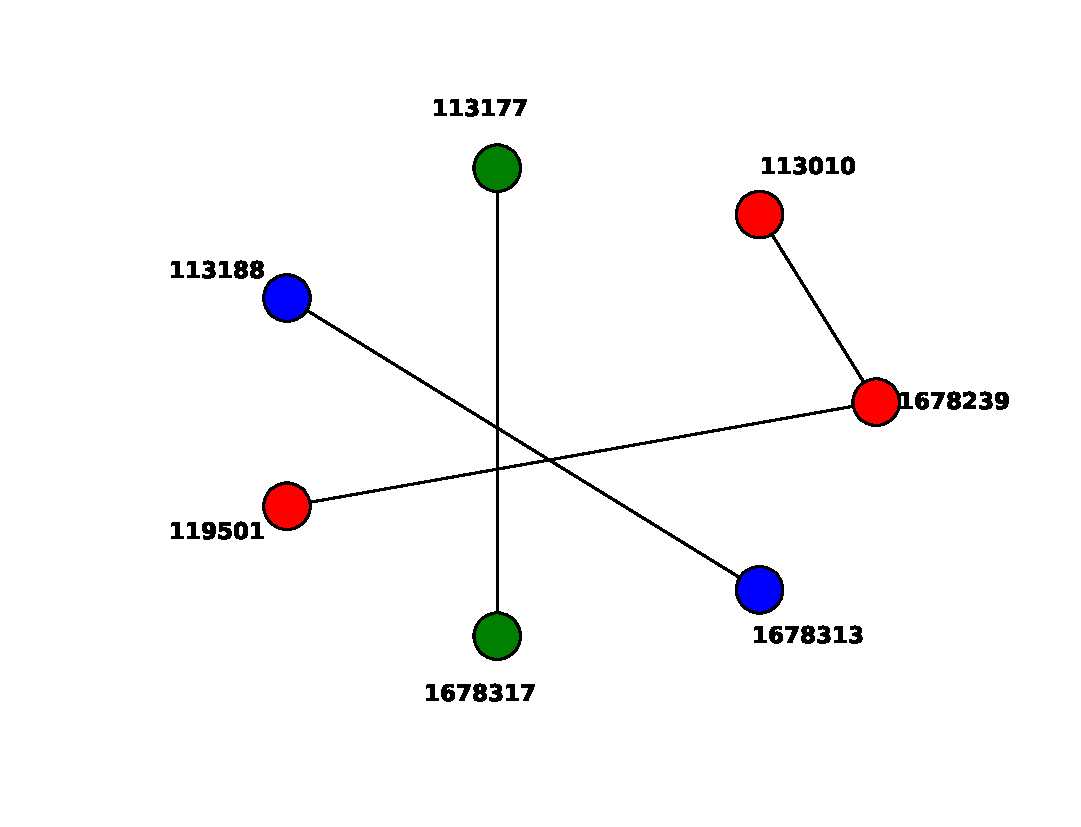
\includegraphics[width=.99\linewidth]{Graphics/Human_Herpesvirus_6Bgraph.eps}
	\caption{A simple PPIN, the one of \textit{Human Herpesvirus 6B}.}
	\label{fig:examplePPIN}
    \vspace{-10pt}
\end{wrapfigure}

\subsubsection*{An Example} Let us focus on \textit{Human Herpesvirus 6B}. After opening this file with a spreadsheet program we can easily observe that the first line (header) contains the labels of columns, followed by four lines with protein-protein interactions. What is more, there are $7$ nodes in total, divided in three components with the largest containing $3$ nodes. This PPIN is depicted in Figure~\ref{fig:examplePPIN} as visualized by \NX. 

In order to create a PPIN, what we need is a type for protein labeling. Given this dataset, there are up to three different ways, for example by using information from \textit{Entrez} database or official symbols. We chose to work with the \textsc{BioGrid} IDs since these labels are numerical and they reference directly to the online repository. 

One drawback of \BGRD is the existence of some noise in the data. By this we mean multiple copies of the same interaction, which corresponds to parallel edges, or even self-loops. In order to remove such entries we used \PY's set datatype which is very efficient. Another part of pre-processing involved a re-labeling of nodes in order to construct necessary tables and arrays easier later on. To make this more helpful, we also saved a dictionary with correspondences between new and initial labels for every organism.  These steps are implemented in script \texttt{ParseBioGridFiles.py} and the functions therein.

\subsection{Basic Information \& Illustration of PPINs}
%\def\rownumber{} % hack for re-starting row-counter (and skip the header) 
\begin{table}[h] %[tbhp]
	\centering
	\caption{\textit{Appendix} - Basic Information about PPINs from \texttt{BioGrid 3.5.165 dataset}}
	\label{table:stats}
    \begin{tabular}{@{\makebox[2em][r]{\rownumber\space}} | lrrcccr}
		\textbf{Organism} & \textbf{\# Nodes} &  \textbf{\# Edges} & \textbf{Avg Degree} & \textbf{ConComps} & \textbf{Largest} & \textbf{Diam} %[0.5ex] 
        \gdef\rownumber{\stepcounter{magicrownumbers}\arabic{magicrownumbers}} \\
		\midrule
        $ Anopheles \ gambiae \ PEST $ & 2 & 1 & 1.00 & 1 & 1.000 & 1 \\ 
        $ Apis \ mellifera $ & 2 & 1 & 1.00 & 1 & 1.000 & 1 \\ 
        $ Arabidopsis \ thaliana \ Columbia $ & 9570 & 35242 & 7.37 & 78 & 0.981 & 12 \\ 
        $ Bacillus \ subtilis \ 168 $ & 2 & 1 & 1.00 & 1 & 1.000 & 1 \\ 
        $ Bos \ taurus $ & 437 & 405 & 1.85 & 73 & 0.162 & 15 \\ 
        $ Caenorhabditis \ elegans $ & 3938 & 7885 & 4.00 & 77 & 0.953 & 13 \\ 
        $ Candida \ albicans \ SC5314 $ & 713 & 860 & 2.41 & 30 & 0.893 & 12 \\ 
        $ Canis \ familiaris $ & 52 & 34 & 1.31 & 20 & 0.135 & 4 \\ 
        $ Cavia \ porcellus $ & 9 & 5 & 1.11 & 4 & 0.333 & 2 \\ 
        $ Chlamydomonas \ reinhardtii $ & 19 & 15 & 1.58 & 4 & 0.632 & 2 \\ 
        $ Chlorocebus \ sabaeus $ & 11 & 7 & 1.27 & 4 & 0.273 & 2 \\ 
        $ Cricetulus \ griseus $ & 32 & 24 & 1.50 & 8 & 0.500 & 3 \\ 
        $ Danio \ rerio $ & 245 & 250 & 2.04 & 37 & 0.404 & 8 \\ 
        $ Dictyostelium \ discoideum \ AX4 $ & 24 & 18 & 1.50 & 6 & 0.208 & 2 \\ 
        $ Drosophila \ melanogaster $ & 9191 & 54806 & 11.93 & 37 & 0.992 & 9 \\ 
        $ Emericella \ nidulans \ FGSC \ A4 $ & 64 & 62 & 1.94 & 6 & 0.703 & 2 \\ 
        $ Equus \ caballus $ & 4 & 2 & 1.00 & 2 & 0.500 & 1 \\ 
        $ Escherichia \ coli \ K12 $ & 2 & 1 & 1.00 & 1 & 1.000 & 1 \\ 
        $ Escherichia \ coli \ K12 \ MC4100 \ BW2952 $ & 10 & 8 & 1.60 & 2 & 0.800 & 6 \\ 
        $ Escherichia \ coli \ K12 \ MG1655 $ & 146 & 127 & 1.74 & 21 & 0.623 & 3 \\ 
        $ Escherichia \ coli \ K12 \ W3110 $ & 4063 & 181620 & 89.40 & 1 & 1.000 & 5 \\ 
        $ Gallus \ gallus $ & 391 & 417 & 2.13 & 42 & 0.588 & 9 \\ 
        $ Glycine \ max $ & 44 & 39 & 1.77 & 7 & 0.318 & 2 \\ 
        $ Hepatitus \ C \ Virus $ & 131 & 129 & 1.97 & 2 & 0.985 & 2 \\ 
        $ Homo \ sapiens $ & 22826 & 318912 & 27.94 & 14 & 0.999 & 9 \\ 
        $ Human \ Herpesvirus \ 1 $ & 174 & 194 & 2.23 & 1 & 1.000 & 8 \\ 
        $ Human \ Herpesvirus \ 2 $ & 7 & 4 & 1.14 & 3 & 0.429 & 2 \\ 
        $ Human \ Herpesvirus \ 3 $ & 4 & 2 & 1.00 & 2 & 0.500 & 1 \\ 
        $ Human \ Herpesvirus \ 4 $ & 240 & 235 & 1.96 & 7 & 0.771 & 8 \\ 
        $ Human \ Herpesvirus \ 5 $ & 91 & 79 & 1.74 & 12 & 0.385 & 4 \\ 
        $ Human \ Herpesvirus \ 6A $ & 11 & 7 & 1.27 & 4 & 0.364 & 2 \\ 
        $ Human \ Herpesvirus \ 6B $ & 7 & 4 & 1.14 & 3 & 0.429 & 2 \\ 
        $ Macaca \ mulatta $ & 15 & 12 & 1.60 & 3 & 0.733 & 2 \\ 
        $ Human \ Herpesvirus \ 7 $ & 2 & 1 & 1.00 & 1 & 1.000 & 1 \\ 
        $ Meleagris \ gallopavo $ & 2 & 1 & 1.00 & 1 & 1.000 & 1 \\ 
        $ Human \ Immunodeficiency \ Virus \ 1 $ & 1121 & 1299 & 2.32 & 1 & 1.000 & 5 \\ 
        $ Human \ Immunodeficiency \ Virus \ 2 $ & 16 & 12 & 1.50 & 4 & 0.500 & 4 \\ 
        $ Human \ papillomavirus \ 16 $ & 14 & 12 & 1.71 & 2 & 0.857 & 4 \\ 
        $ Mus \ musculus $ & 13003 & 38624 & 5.94 & 89 & 0.984 & 15 \\ 
        $ Neurospora \ crassa \ OR74A $ & 12 & 10 & 1.67 & 2 & 0.667 & 2 \\ 
        $ Mycobacterium \ tuberculosis \ H37Rv $ & 11 & 9 & 1.64 & 2 & 0.818 & 2 \\ 
        $ Nicotiana \ tomentosiformis $ & 2 & 1 & 1.00 & 1 & 1.000 & 1 \\ 
        $ Oryctolagus \ cuniculus $ & 283 & 271 & 1.92 & 33 & 0.502 & 9 \\ 
        $ Oryza \ sativa \ Japonica $ & 74 & 90 & 2.43 & 18 & 0.351 & 3 \\ 
        $ Pan \ troglodytes $ & 10 & 5 & 1.00 & 5 & 0.200 & 1 \\ 
        $ Ovis \ aries $ & 2 & 1 & 1.00 & 1 & 1.000 & 1 \\ 
        $ Pediculus \ humanus $ & 2 & 1 & 1.00 & 1 & 1.000 & 1 \\ 
        $ Plasmodium \ falciparum \ 3D7 $ & 1224 & 2445 & 4.00 & 23 & 0.963 & 10 \\ 
        $ Rattus \ norvegicus $ & 3713 & 5227 & 2.82 & 118 & 0.918 & 14 \\ 
        $ Ricinus \ communis $ & 3 & 2 & 1.33 & 1 & 1.000 & 2 \\ 
        $ Saccharomyces \ cerevisiae \ S288c $ & 7158 & 534073 & 149.22 & 1 & 1.000 & 6 \\ 
        $ Schizosaccharomyces \ pombe \ 972h $ & 4292 & 58217 & 27.13 & 7 & 0.997 & 8 \\ 
        $ Selaginella \ moellendorffii $ & 6 & 8 & 2.67 & 1 & 1.000 & 2 \\ 
        $ Simian \ Immunodeficiency \ Virus $ & 19 & 16 & 1.68 & 4 & 0.421 & 3 \\ 
        $ Simian \ Virus \ 40 $ & 6 & 5 & 1.67 & 1 & 1.000 & 2 \\ 
        $ Solanum \ lycopersicum $ & 45 & 96 & 4.27 & 7 & 0.467 & 4 \\ 
        $ Solanum \ tuberosum $ & 4 & 2 & 1.00 & 2 & 0.500 & 1 \\ 
        $ Sus \ scrofa $ & 94 & 79 & 1.68 & 23 & 0.234 & 5 \\ 
        $ Strongylocentrotus \ purpuratus $ & 17 & 16 & 1.88 & 1 & 1.000 & 2 \\ 
        $ Vaccinia \ Virus $ & 8 & 5 & 1.25 & 3 & 0.375 & 2 \\ 
        $ Tobacco \ Mosaic \ Virus $ & 3 & 2 & 1.33 & 1 & 1.000 & 2 \\ 
        $ Ustilago \ maydis \ 521 $ & 4 & 3 & 1.50 & 1 & 1.000 & 2 \\ 
        $ Xenopus \ laevis $ & 1128 & 1212 & 2.15 & 61 & 0.850 & 15 \\ 
        $ Vitis \ vinifera $ & 2 & 1 & 1.00 & 1 & 1.000 & 1 \\ 
        $ Zea \ mays $ & 21 & 11 & 1.05 & 10 & 0.143 & 2 \\ 
        $ Human \ Herpesvirus \ 8 $ & 714 & 687 & 1.92 & 45 & 0.529 & 12 \\ 
                %[1ex] 
		\bottomrule
    \end{tabular}
	%\addtabletext{nomenclature for the TSs refers to the numbered species in the table.}
\end{table}
The first step of the analysis was the calculation of some fundamental properties for each PPIN, i.e. number of nodes ($N$), number of edges ($M$), average degree of nodes, number of connected components, relative size of largest connected component (LGC) and diameter. The later is computed for the LGC, for disconnected cases.  All these are summarized in Table~\ref{table:stats} (\textit{Appendix}). 

Interestingly, the majority of small PPINs, i.e. those with only a few hundreds of nodes or less, show low connectivity. Two characteristic examples are \textit{Bos taurus} (cattle) or \textit{Danio rerio} (zebrafish) whose largest connected component contains $16\%$ and $40\%$, respectively, of the total nodes. Larger networks, on the contrary, show a very different behavior regarding connectivity; almost every PPIN containing thousands of nodes has a giant component containing more than $90\%$ of nodes. One such notable example is that of \textit{Human Immunodeficiency Virus 1}, which is fully connected, illustrated Figure~\ref{fig:HIV}. 

\begin{figure}
  \centering
  \vspace{-70pt}
  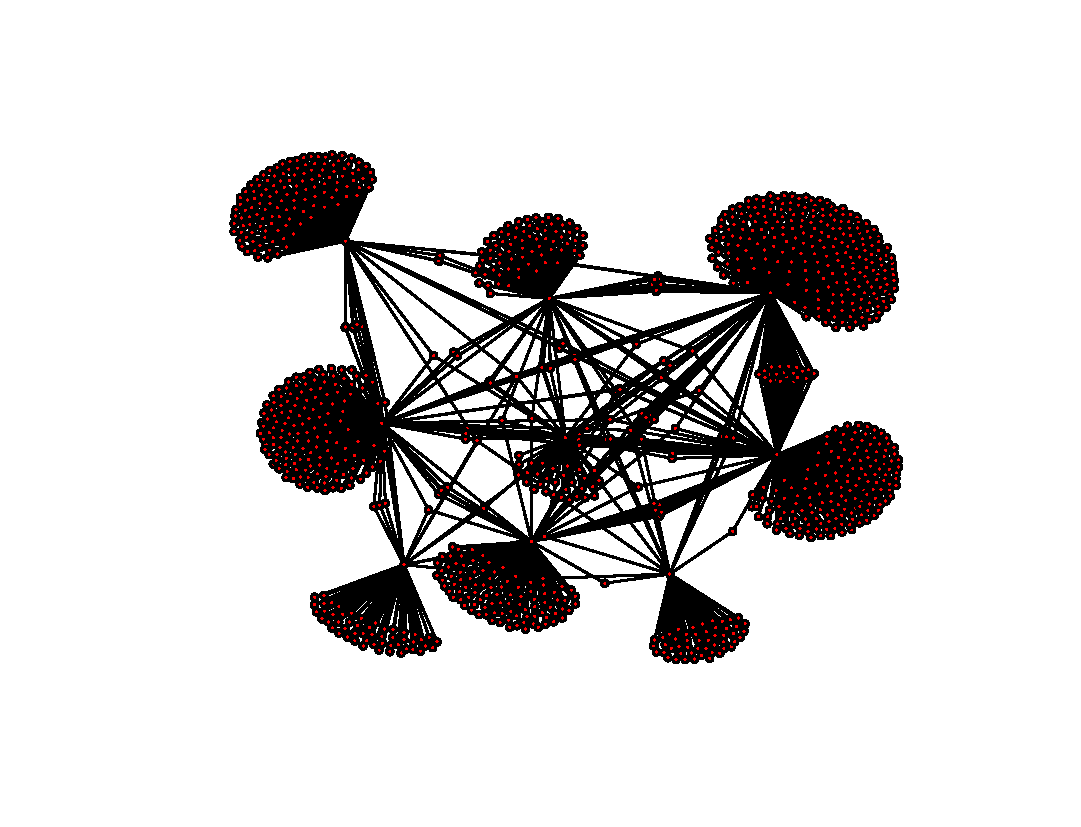
\includegraphics[width=.99\linewidth]{Graphics/Human_Immunodeficiency_Virus_1graph.eps}
  \vspace{-30pt}
  \caption{PPIN of \textit{Human Immunodeficiency Virus 1}.}
  \label{fig:HIV}
\end{figure}

\subsection{Centrality \& Important Proteins}
One of the most useful tasks in Network Science is the location of the most central or important nodes. This has always been of high importance in many scientific fields with a seminal work from Sociology aging more than six decades~\cite{katz1953new}. After the enormous expansion of World Wide Web and the need of finding meaningful websites efficiently, the field of Node Ranking has gained a lot of attention the last two decades \cite{langville2011google}. To date, there is a variety of algorithms that measure centrality in order to estimate the most important ones, each with specific advantages, but also drawbacks, regarding speed, accuracy and the need of resources.   

\NX, in particular, has a lot of built-in algorithms for node centrality, some of which we used for the analysis. First of all, \texttt{Degree Centrality} is by far an easy to compute measure and yet meaningful as it considers every direct interaction. \texttt{Katz Index} and \texttt{HITS} are algorithms that place emphasis on indirect connections. \texttt{PageRank} does also the same but in a more computationally efficient way as it incorporates many tools. The last measure we are using is \texttt{Closeness Centrality} which corresponds to the reciprocal of the average distance of a node to every other. A lot of PPINs are divided in connected components which would result in frailty when calculating closeness as some distances would be equal to infinity. To overcome this obstacle, closeness centrality is defined by an improved formula~\cite{wasserman1994social} as
\begin{equation}
	C(u) = \frac{n-1}{N-1} \frac{n - 1}{\sum_{v=1}^{n-1} d(v, u)},
\end{equation}
where n is the size of the related component and $d(u,v)$ is shortest path (i.e. the distance) between nodes $u$ and $v$. Calculating the aforementioned distances is a difficult task, however, since this is part of the next task in the project (see Section~\ref{sec:3-task2}), we implemented a new function that calculates the closeness centralities, given the distances (check function \texttt{MyCloseness} in \texttt{PPINutils.py} script). \texttt{PageRank} and \texttt{HITS} are implemented by \NX in an optimal way (\textit{scipy versions}) which, even for the largest PPINs needed only a few seconds of running time. \texttt{Katz}, on the other hand, requires the solution of a system of linear equations (or the inversion of a huge matrix otherwise), which is very time-consuming. We also tried to compute the \texttt{Betweenness Centrality} but without success, due to the high demand of processing resources.

We are now focusing on \textit{Homo sapiens}, a PPIN with $22826$ nodes, for the estimation of the most central proteins. On a typical DTC computer ($3.50$ GHz and $7.7$ GB of RAM), \texttt{PageRank} and \texttt{Degree Centrality} took less than two seconds to run and \texttt{HITS} required approximately ten seconds. Closeness centralities were computed in almost three minutes and, finally, \texttt{Katz} took more than $45$ minutes. Some of the resulting rankings seem to be consistent whereas other are dissimilar. For instance, \texttt{HITS} ``agrees'' with \texttt{PageRank} by $TODO$ counted by Spearmann's $\rho$ ranking coefficient. 

In order to select the most important nodes we do the following procedure: we select the top-$15$ ranked nodes by each of the five algorithms, create a list with all these $75$ elements and count the multiple occurrences. The most frequent proteins are reported in Table~\ref{tab:central} accompanied by the corresponding gene and protein function. 


\begin{table}[h]%[tbhp]
	\centering
	\caption{Top-5 Central Proteins in \textit{Homo Sapiens}}
	\begin{tabular}{cccl}
		Node Label & Protein & Gene & Function \\
		\midrule
		114030 & Cullin-3 & CUL3 & This protein plays a critical role in the polyubiquitination and subsequent degradation of specific protein substrates \\
		113164 & HMG20 &  UBC & It plays a key role in maintaining cellular ubiquitin levels under stress. Defects could lead to embryonic lethality. \\
		108309 & HuR & ELAVL1 & RNA-binding protein that binds to the 3'-UTR region of mRNAs and increases their stability \\
		113348 & Exportin-1 & XPO1 &  eukaryotic protein that mediates the nuclear export of proteins, rRNA, snRNA, and some mRNA. \\
		113010 & TP53 & TP53 & tumor suppressor protein containing transcriptional activation, DNA binding, and oligomerization domains.  \\
		%\[ 114030,\ 113164,\ 108309,\ 113348,\ 113010. \]
        \bottomrule
		\label{tab:central}
	\end{tabular}
\end{table}

\subsection{Degree Distributions}

We move to another interesting aspect of complex networks which concerns the distribution of degrees. Although many of the constructed PPINs are interesting, for the sake of clarity we focus mainly on those by \textit{Homo sapiens} and HIV. We present such information in Figures~\ref{fig:DD_Hs}-\ref{fig:DD_HIV}. In general, as was also mentioned in Section~\ref{SS:Intro}, most of the PPINs are scale-free since there are hubs that are connected with a large proportion of nodes and, on the same time, a lot of nodes have only a few edges. This behavior, which is explained by the fact that degree distributions of such networks usually follow a power-law \cite{barabasi2003scale}, can be observed by the histograms (left part of the following figures).  

\begin{figure}[h]
	\begin{minipage}{0.51\textwidth}
		%\flushleft
		%\centering
		%\vspace{0pt}
		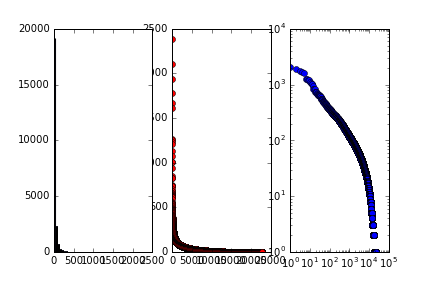
\includegraphics[width=\textwidth]{Graphics/Homo_sapiens-DD.png}
        \caption{Degree distribution in \textit{Homo sapiens}}
        \label{fig:DD_Hs}
	\end{minipage}
	%\hfill
	\begin{minipage}{0.51\textwidth}
		\flushleft
		%\vspace{10pt} % Hack for correct positioning
		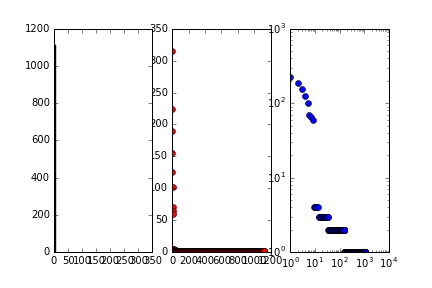
\includegraphics[width=\textwidth]{Graphics/Human_Immunodeficiency_Virus_1-DD}
		%\caption{{\small Graphical representation of }} 
        \caption{Degree distribution in \textit{HIV-1}}
		\label{fig:DD_HIV}
	\end{minipage}
\end{figure}

\subsection{Computational Complexity}
We are now investigating the time complexity for PPIN construction. There might be a variety of different ways  to study complexity but we measure the total time needed for loading an edge-file with \PY and adding the set of edges in a \NX graph. We assume that intermediate actions are the same for every organism and try to find a more abstract relationship between time ($T$) and size of graphs ($N or M$).

After measuring the time complexity for each of the  $66$ cases, we construct two plots in a logarithmic scale, as presented in Figures~\ref{fig:TimeVsEdges}-\ref{fig:TimeVsNodes}. We also plot a corresponding line after fitting a linear regression model. Despite the existence of some oscillations in small graphs, there seems to be a strong linear relationship between $T$ and $M$ and a less accurate linearity between $T$ and $N$. Speeding-up the construction of PPINs would require a deeper understanding of \PY's commands for file I/O. For instance, working with \texttt{Pandas} module instead of \texttt{csv.reader} gives a high advantage when constructing a graph from the scratch. On the other hand, we noticed that \texttt{csv.reader} was the only feasible way to read large files with node-distances. 

\begin{figure}[h]
	\begin{minipage}{0.51\textwidth}
		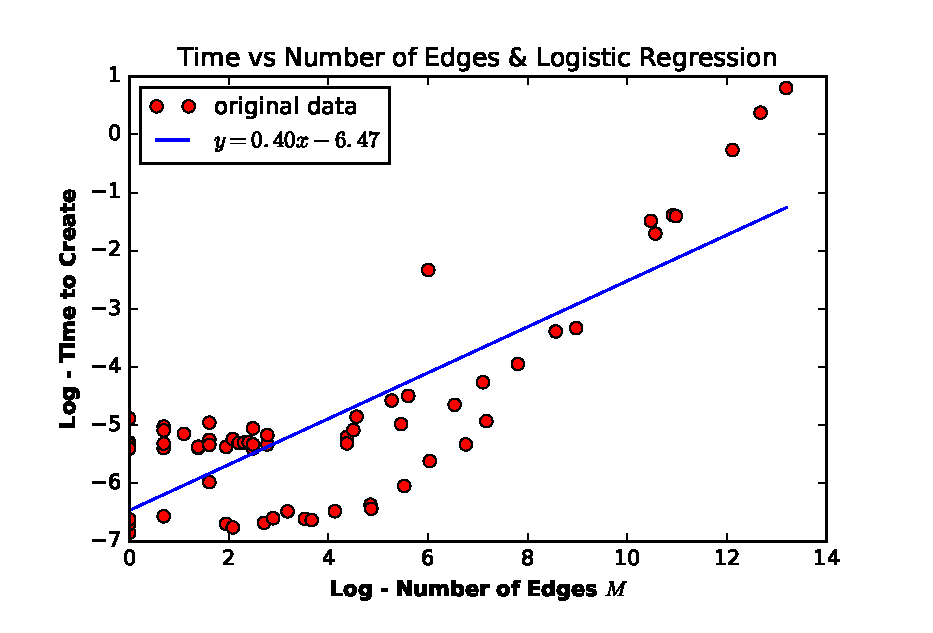
\includegraphics[width=\textwidth]{Graphics/TimeVsEdges.eps}
        \caption{Time vs Number of Edges}
        \label{fig:TimeVsEdges}
	\end{minipage}
	%\hfill
	\begin{minipage}{0.51\textwidth}
		\flushleft
		%\vspace{10pt} % Hack for correct positioning
		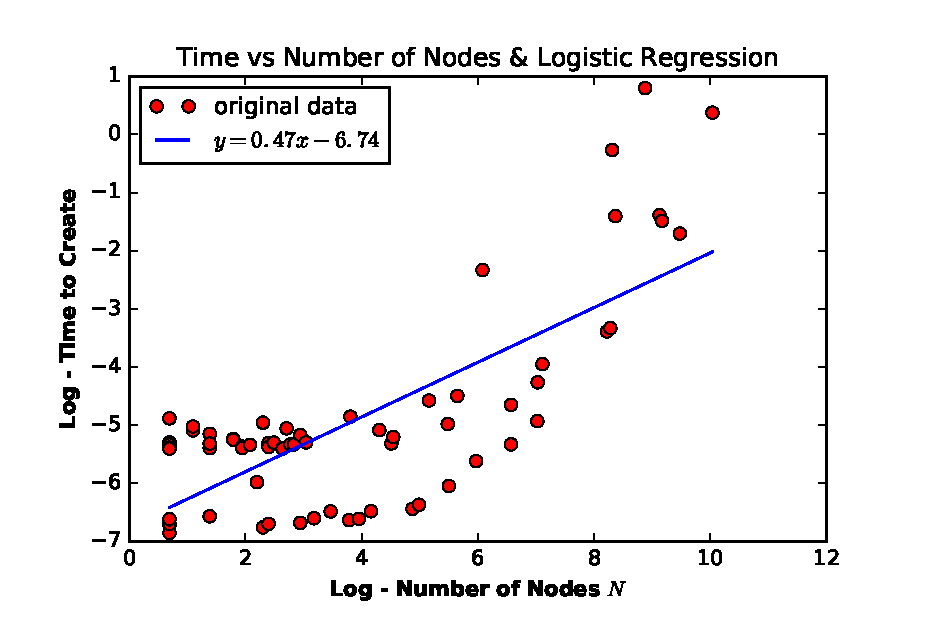
\includegraphics[width=\textwidth]{Graphics/TimeVsNodes.eps}
        \caption{Time vs Number of Nodes}
		\label{fig:TimeVsNodes}
	\end{minipage}
\end{figure}

%\subsection{Opt: The Development of PPINs} 